% Permission is granted to copy, distribute and/or modify this document
% under the terms of the GNU Free Documentation License, Version 1.2
% or any later version published by the Free Software Foundation;
% with no Invariant Sections, no Front-Cover Texts, and no Back-Cover
% Texts.  A copy of the license is included in the section entitled "GNU
% Free Documentation License".
% Copyright 2014 EDF
%

%%%%%%%%%%%%%%%%%%%%%%%%%%%%%%%%%%%%%%%%%%%%%%%%%%%%%%%%%%%%%%%%%%%%%%%%%%%%%%%%%%%%%%%%%%
\section{Use Cases Guide}

This section presents the main functionalities of the module \textit{otlhs} in their context.\\

%%%%%%%%%%%%%%%%%%%%%%%%%%%%%%%%%%%%%%%%%%%%%%%%%%%%%%%%%%%%%%%%%%%%%%%%%%%%%%%%%%%%%%%%%%
\subsection{Latin Hypercube Sample}

Class \texttt{LHSDesign} builds designs of a fixed size, type and bounds. Comparing to the \texttt{LHSExperiment} of the \texttt{OpenTURNS} library, when regenerating sample, the cells selection changes.\\

Python script for this use case:

\begin{lstlisting}
import openturns as ot
import otlhs
#  Generating a design of size N=100
N = 100
# Considering independent Uniform distributions of dimension 3
# Bounds are (-1,1), (0,2) and (0, 0.5)
bounds = ot.Interval([-1,0,0], [1,2,0.5])
# Random LHS
lhs_random = otlhs.LHSDesign(bounds, N)
randomLHS = lhs_random.generate()
# Centered LHS
lhs_centered = otlhs.LHSDesign(bounds, N, True)
centeredLHS = lhs_centered.generate()
print(centeredLHS)
\end{lstlisting}

%%%%%%%%%%%%%%%%%%%%%%%%%%%%%%%%%%%%%%%%%%%%%%%%%%%%%%%%%%%%%%%%%%%%%%%%%%%%%%%%%%%%%%%%%%
\subsection{Plot of LHS}

Class \texttt{PlotDesign} helps to plot a LHS design and draw it in a PDF, PNG, EPS or FIG formats.\\

Python script for this use case:

\begin{lstlisting}
import openturns as ot
import otlhs
#  Generating a design of size N=10
N = 10
# Considering independent Uniform distributions of dimension 3
# Bounds are (-1,1), (0,2) and (0, 0.5)
bounds = ot.Interval([-1,0,0], [1,2,0.5])
# Centered LHS
lhs_centered = otlhs.LHSDesign(bounds, N, True)
centeredLHS = lhs_centered.generate()
# Draw the design + grids
drawable = otlhs.PlotDesign(centeredLHS, bounds, 10, 10)
# This is equivalent to:
# drawable = otlhs.PlotDesign(centeredLHS, bounds)
# Create ot graph
graph = ot.Graph()
# Add drawable
graph.add(drawable)
# Export into PDF file. Refer to Graph class
graph.draw("design", 640, 480, ot.GraphImplementation.PDF)
\end{lstlisting}

Notice that there is no <<show method>> for that class. An alternative is to use the \texttt{PyPlotDesign} class.
This requires the \texttt{matplotlib} module.\\

Python script for this use case:

\begin{lstlisting}
import openturns as ot
import otlhs
from otlhs.pyplotdesign import PyPlotDesign
import matplotlib.pylab as plt
#  Generating a design of size N=10
N = 10
# Considering independent Uniform distributions of dimension 3
# Bounds are (-1,1), (0,2) and (0, 0.5)
bounds = ot.Interval([-1,0,0], [1,2,0.5])
# Centered LHS
lhs_centered = otlhs.LHSDesign(bounds, N, True)
centeredLHS = lhs_centered.generate()
# Draw design and grid
plot = PyPlotDesign(centeredLHS, bounds, 10, 10)
# Show the graph
plt.show()
# Export the graph
plot.savefig("design.png")
\end{lstlisting}

%%%%%%%%%%%%%%%%%%%%%%%%%%%%%%%%%%%%%%%%%%%%%%%%%%%%%%%%%%%%%%%%%%%%%%%%%%%%%%%%%%%%%%%%%%

\subsection{LHS and space filling}

\texttt{SpaceFilling} is an abstract class to compute the criterion value of a given design. \texttt{SpaceFillingC2} and \texttt{SpaceFillingPhiP} are implemented here.
Note that these classes support only the computation of the criterion, and not its optimization.\\

Python script for this use case:

\begin{lstlisting}
import openturns as ot
import otlhs
#  Generating a design of size N=100
N = 100
# Considering independent Uniform distributions of dimension 3
# Bounds are (-1,1), (0,2) and (0, 0.5)
bounds = ot.Interval([-1,0,0], [1,2,0.5])
# Random LHS
lhs = otlhs.LHSDesign(bounds, N)
design = lhs.generate()
# C2
c2 = otlhs.SpaceFillingC2().evaluate(design)
# PhiP with default p
phip = otlhs.SpaceFillingPhiP().evaluate(design)
# mindist
mindist = otlhs.SpaceFillingMinDist().evaluate(design)
# For p->infinity
phip_inf = otlhs.SpaceFillingPhiP(100).evaluate(design)
\end{lstlisting}

%%%%%%%%%%%%%%%%%%%%%%%%%%%%%%%%%%%%%%%%%%%%%%%%%%%%%%%%%%%%%%%%%%%%%%%%%%%%%%%%%%%%%%%%%%
\subsection{Optimized LHS using Monte Carlo}
Given a space filling criterion, it is possible to generate many designs and to return the ``best'' one. This method is trivial to implement but the number of generations may become impractical.\\

The class \texttt{MonteCarloLHS} gives the optimal design using the \texttt{LHSDesign} as factory and number of simulations.
Default space filling criterion is \texttt{SpaceFillingMinDist}.\\
Python script for this use case:

\begin{lstlisting}
import openturns as ot
import otlhs

# Considering independent Uniform(0,1) distributions of dimension 3
bounds = ot.Interval(3)
designSize = 100
# Random LHS MonteCarlo
lhs = otlhs.LHSDesign(bounds, designSize)
# MonteCarlo, with nSimu=50000 and default space_filling
nSimu = 50000
algo = otlhs.MonteCarloLHS(lhs, nSimu)
result = algo.generate()
# optimal design
design = result.getOptimalDesign()
\end{lstlisting}

Results may be completed by the fixed criterion value history for all samples, the final criteria values.\\
Python script for this use case:
\begin{lstlisting}
import openturns as ot
import otlhs
#  Generating a design of size N=100
N = 100
# Considering independent Uniform distributions of dimension 3
# Bounds are (-1,1), (0,2) and (0, 0.5)
bounds = ot.Interval([-1,0,0], [1,2,0.5])
# Random LHS MonteCarlo
lhs = otlhs.LHSDesign(bounds, N)
# Fixing C2 crit
space_filling = otlhs.SpaceFillingC2()
# Defining MonteCarlo, with nSimu=50000
nSimu = 50000
algo = otlhs.MonteCarloLHS(lhs, nSimu, space_filling)
result = algo.generate()
# optimal design
design = result.getOptimalDesign()
history = result.getAlgoHistory()
# Final criteria values
c2 = result.getC2()
phip = result.getPhiP()
mindist = result.getMinDist()
\end{lstlisting}

%%%%%%%%%%%%%%%%%%%%%%%%%%%%%%%%%%%%%%%%%%%%%%%%%%%%%%%%%%%%%%%%%%%%%%%%%%%%%%%%%%%%%%%%%%
\subsection{Optimized LHS using simulated annealing}
As with Monte Carlo, user decides of a fixed number of iterations, but this time this number is part of the temperature profile.  Two profiles are currently provided:
\begin{itemize}
\item Linear profile: $T(i) = T(0) \left( 1 - \frac{i}{nrIter} \right)$
\item Geometric profile: $T(i) = T(0) c^i,\; 0 < c < 1$.
\end{itemize}

Starting from an LHS design, a new design is built by permuting a random coordinate of two randomly chosen sample points; this new design is also an LHS. but not necessary a ``more efficient'' design.
A comparison of criteria of the two designs is done, and the new LHS is accepted with probability
\begin{equation*}
min\left(exp\left[ -\frac{ \phi(\text{LHSnew}) - \phi(\text{LHS})}{T(i)} \right], 1\right)
\end{equation*}

The simulated annealing algorithm is detailed in Algorithm \ref{algo_simu_annealing}.\\

Minimal python script for the use case:
\begin{lstlisting}
import openturns as ot
import otlhs
designSize = 100
# Considering independent Uniform(0,1) distributions of dimension 3
bounds = ot.Interval(3)
# Random LHS
lhs = otlhs.LHSDesign(bounds, N)
algo = otlhs.SimulatedAnnealingLHS(lhs)
result = algo.generate()
# Retrieve optimal design
design = result.getOptimalDesign()
\end{lstlisting}

One could also fix the criterion, the temperature profile and gets more results.

Python script for this use case:
\begin{lstlisting}
import openturns as ot
import otlhs
#  Generating a design of size N=100
N = 100
# Considering independent Uniform distributions of dimension 3
# Bounds are (-1,1), (0,2) and (0, 0.5)
bounds = ot.Interval([-1,0,0], [1,2,0.5])
# Random LHS
lhs = otlhs.LHSDesign(bounds, N)
# Fixing C2 crit
space_filling = otlhs.SpaceFillingC2()
# Defining a temperature profile
# A geometric profile seems accurate with default parameters
# e.g. T0=10, c=0.95, iMax=2000
temperatureProfile = otlhs.GeometricProfile()
algo = otlhs.SimulatedAnnealingLHS(lhs, temperatureProfile, space_filling)
result = algo.generate()
# Retrieve optimal design
design = result.getOptimalDesign()
# Criteria for the optimal design
crit_c2 = result.getC2()
crit_phip = result.getPhiP()
crit_mindist = result.getMinDist()
# History of the criterion used for optimization
history = result.getAlgoHistory()
criterion_hist = history[:, 0]
# Additional results
temperature_hist = history[:, 1]
probability_hist = history[:, 2]
\end{lstlisting}

It is also possible to chain several iterations of the whole process with different starting points.
Python script for this use case:
\begin{lstlisting}
import openturns as ot
import otlhs
#  Generating a design of size N=100
N = 100
# Considering independent Uniform distributions of dimension 3
# Bounds are (-1,1), (0,2) and (0, 0.5)
bounds = ot.Interval([-1,0,0], [1,2,0.5])
# Random LHS
lhs = otlhs.LHSDesign(bounds, N)
# Fixing PhiP crit
space_filling = otlhs.SpaceFillingPhiP()
# Defining a temperature profile
# T0=10, iMax=3000
temperatureProfile = otlhs.LinearProfile(10.0, 3000)
algo = otlhs.SimulatedAnnealingLHS(lhs, temperatureProfile, space_filling)
restart = 50
result = algo.generate(restart)
# Retrieve optimal design
design = result.getOptimalDesign()
# Retrieve all optimal designs
designs = [result.getOptimalDesign(i) for i in xrange(restart)]
\end{lstlisting}

Finally, we could start the optimization process of LHS using a precomputed LHS design.
Python script for this use case:
\begin{lstlisting}
import openturns as ot
import otlhs
#  Generating a design of size N=100
N = 100
# Considering independent Uniform distributions of dimension 3
# Bounds are (0,1)^3
bounds = ot.Interval(3)
# Random LHS
lhs = otlhs.LHSDesign(bounds, N)
# Fixing C2 crit for example
space_filling = otlhs.SpaceFillingC2()
# Defining a temperature profile
# T0=10, iMax=3000
temperatureProfile = otlhs.LinearProfile(10.0, 3000)
algo = otlhs.SimulatedAnnealingLHS(lhs, temperatureProfile, space_filling)
result = algo.generate()
# optimal design
design = result.getOptimalDesign()
# check history ==> draw criterion
ot.Show( result.drawHistoryCriterion() )
# Convergence needs to be performed
# New algo starting from this design
algo = otlhs.SimulatedAnnealingLHS(design, bounds, temperatureProfile, space_filling)
result = algo.generate()
# New design
design = result.getOptimalDesign()
\end{lstlisting}


\subsection{Ishigami test}
The following example illustrates the generation of an optimal design for surrogate model learning purposes.
The use case proposed here is the Ishigami function. The model requires $3$ input parameters, which are known to be
uniformly distributed in $[-\pi,\pi]^3$.\\

Python script for a detailed study is proposed hereafter:

\lstinputlisting[language=Python]{ishigami_test.py}

We illustrate hereafter the design obtained that optimize the $C_2$ criterion in figure \ref{design_ishigami}.
\begin{figure}[!h]
\label{design_ishigami}
 \begin{center}
  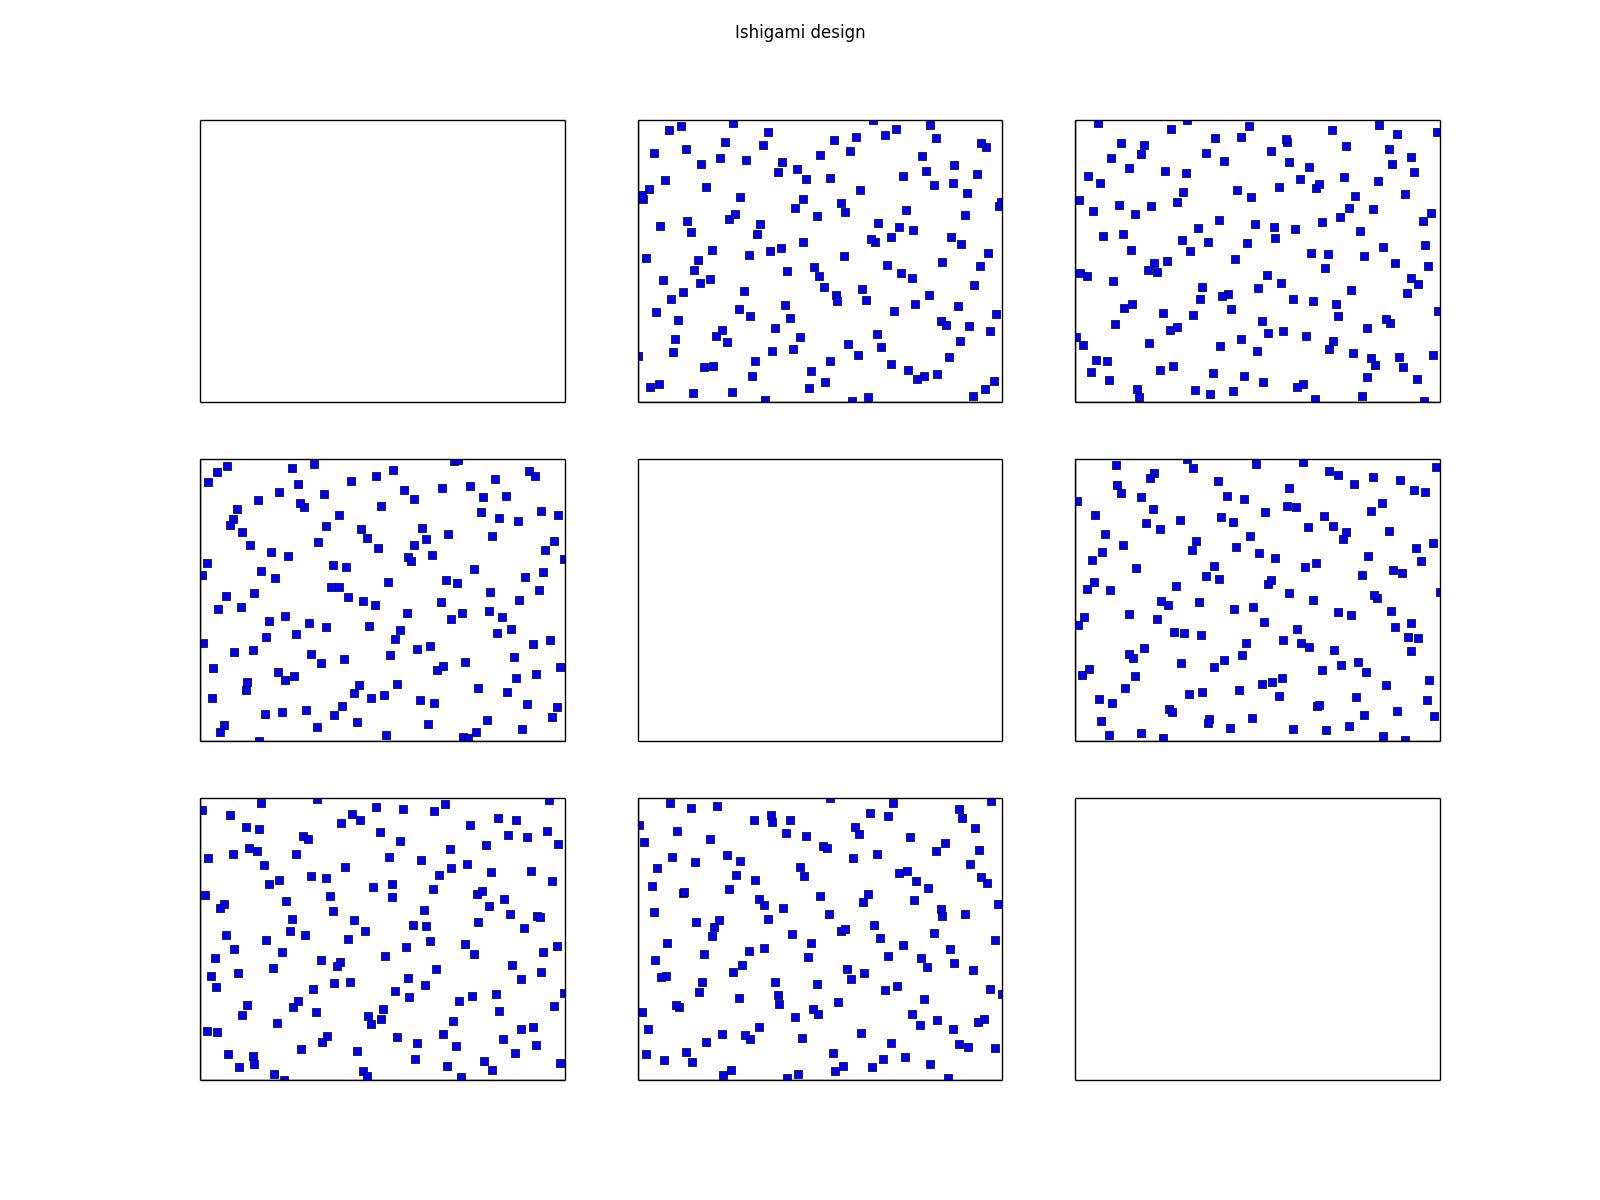
\includegraphics[scale=0.25]{design_ishigami.png}
 \end{center}
 \caption{Input design for learning Ishigami model}
\end{figure}
\newpage The design seems accurate. To complete this example, the validation using an independent validation sample is done as illustrated in figure \ref{ishigami_model_validation}

\begin{figure}[!h]\label{ishigami_model_validation}
 \begin{center}
  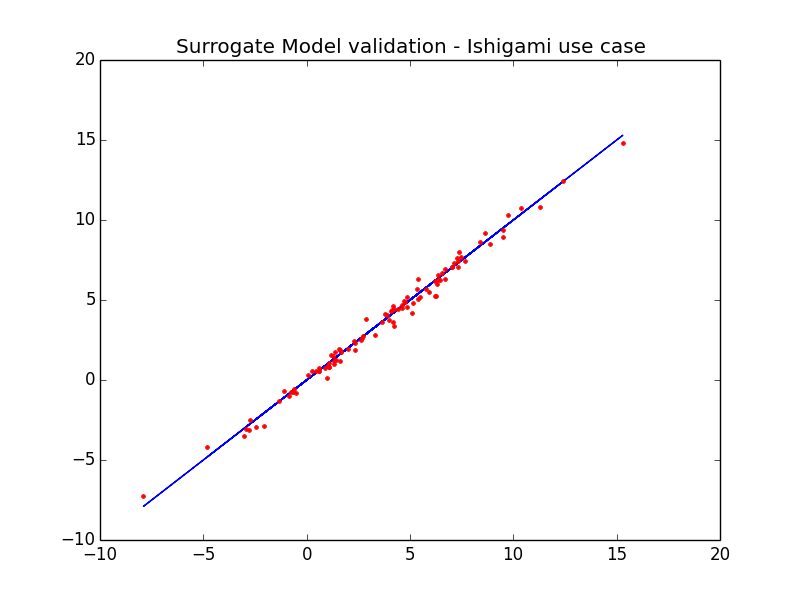
\includegraphics[scale=0.35]{ishigami_model_validation.png}
 \end{center}
 \caption{Validation of surrogate model}
\end{figure}
